\documentclass{report}

\usepackage{hyperref} % makes ToC clickable

% \usepackage{dnd}
\usepackage{eso-pic} % allows background picture patterning
\usepackage{graphicx} % \includegraphics
\usepackage[left=1in,top=1in,right=1in,nohead]{geometry}
% \usepackage{color} % Color DM only stuff
\usepackage{xcolor}
\usepackage{mdframed}
\usepackage{multicol}
\usepackage{tipa} % Ezh = \textyogh
\usepackage{etoolbox} % \ifdef / \ifundef for setting
\usepackage{fp} % For simple arithmetic / mod calculation
\usepackage{amsmath}
\usepackage{textcomp} % \textrightarrow
\hypersetup{
  colorlinks,
  linktoc=all,
  linkcolor=blue,
  urlcolor=black
}

\usepackage[colorinlistoftodos,prependcaption,textsize=tiny]{todonotes}   % adds \todo

\newif\ifdm
\dmtrue

\let\stdsection\section
\renewcommand{\section}{\clearpage\stdsection}

\newcommand{\dmonly}[1]{\ifdm{\color{blue}\hrulefill\par\textit{DM Only} #1\par\hrulefill}\else{}\fi}

\newcommand{\headeritem}[2]{\textbf{#1:} #2}

\newcommand{\race}[1]{\headeritem{Race}{#1}}
\newcommand{\class}[1]{\headeritem{Class}{#1}}
\newcommand{\voice}[1]{\headeritem{Voice}{#1}}
\newcommand{\player}[1]{\headeritem{Player}{#1}}

\newcommand{\STR}[1]{\renewcommand{\StrVal}{#1}}
\newcommand{\DEX}[1]{\renewcommand{\DexVal}{#1}}
\newcommand{\CON}[1]{\renewcommand{\ConVal}{#1}}
\newcommand{\INT}[1]{\renewcommand{\IntVal}{#1}}
\newcommand{\WIS}[1]{\renewcommand{\WisVal}{#1}}
\newcommand{\CHA}[1]{\renewcommand{\ChaVal}{#1}}

\newcommand{\statblock}[6]{\STR{#1}\DEX{#2}\CON{#3}\INT{#4}\WIS{#5}\CHA{#6}}

\newcommand{\modOf}[1]{%
\FPupn\unrounded{10.1 #1 - 2 swap /}%
\FPround\rounded\unrounded0%
\FPclip\result\rounded%
\FPifneg\result{%
\FPabs\absresult\result%
\FPround\rounded\absresult0%
\FPclip\newresult\rounded%
\texttt{-}\newresult%
}\else{%
\texttt{+}\result}\fi%
}

\newcommand{\reset}{
  \def\StrVal\undefined
  \def\DexVal\undefined
  \def\ConVal\undefined
  \def\IntVal\undefined
  \def\WisVal\undefined
  \def\ChaVal\undefined
}

\newcommand{\makeCharacterHeader}{%
  \begin{tabular}{cccccc}
    \stackrel{STR}{\StrVal(\modOf{\StrVal})} &
    \stackrel{DEX}{\DexVal(\modOf{\DexVal})} &
    \stackrel{CON}{\ConVal(\modOf{\ConVal})} &
    \stackrel{INT}{\IntVal(\modOf{\IntVal})} &
    \stackrel{WIS}{\WisVal(\modOf{\WisVal})} &
    \stackrel{CHA}{\ChaVal(\modOf{\ChaVal})}
  \end{tabular}
}

% \newenvironment{name}[args][default]{before}{after}
\newenvironment{aloud}{%
\begin{quote}%
\begin{sl}%
\begin{mdframed}[backgroundcolor=blue!10]
}{%
\end{mdframed}%
\end{sl}%
\end{quote}%
}
\newenvironment{character}[1]{
  \section{#1}
}{\reset}

\def\[#1\]{%
\begin{aloud}#1\end{align}%
}


\newcommand{\Enyhito}{Enyh\'{\i}t\H{o}}

\begin{document}

  \dmonly{{\LARGE
    This is the DM copy.
    If you're a player, this will have spoilers.
  }}

  \AddToShipoutPictureBG{
\includegraphics{parchment-paper-light-texture.png}}

  \tableofcontents

  \chapter{Foreword: Mechanics and Meta-information}

\section{Damage description}

Generally, I will call for you to describe your attacks hit.
However, in a fight it really only takes one or two solid hits with a weapon to kill someone.
To keep things at least half sensible with respect to how much damage a monster can soak, I'll use
  the following general guides when calling for the severity of blow your just dealt.

\begin{tabular}{|r|l|}
\hline
Remaining HP\dots & Described as \\
\hline
$0\%$    & Killing \\
$<25\%$  & Wounding \\
$<50\%$  & Connecting \\
$<75\%$  & Glancing \\
$<100\%$ & Absorbed \\
\hline
\end{tabular}

\newpage
\section{Speed Factor Initiative}

I'd like to use the Speed Factor Initiative rules with the Angry DM's modifier table.

For more, read:\newline\url{http://theangrygm.com/fine-i-wrote-about-speed-factor-initiative-in-dd-5e/}.

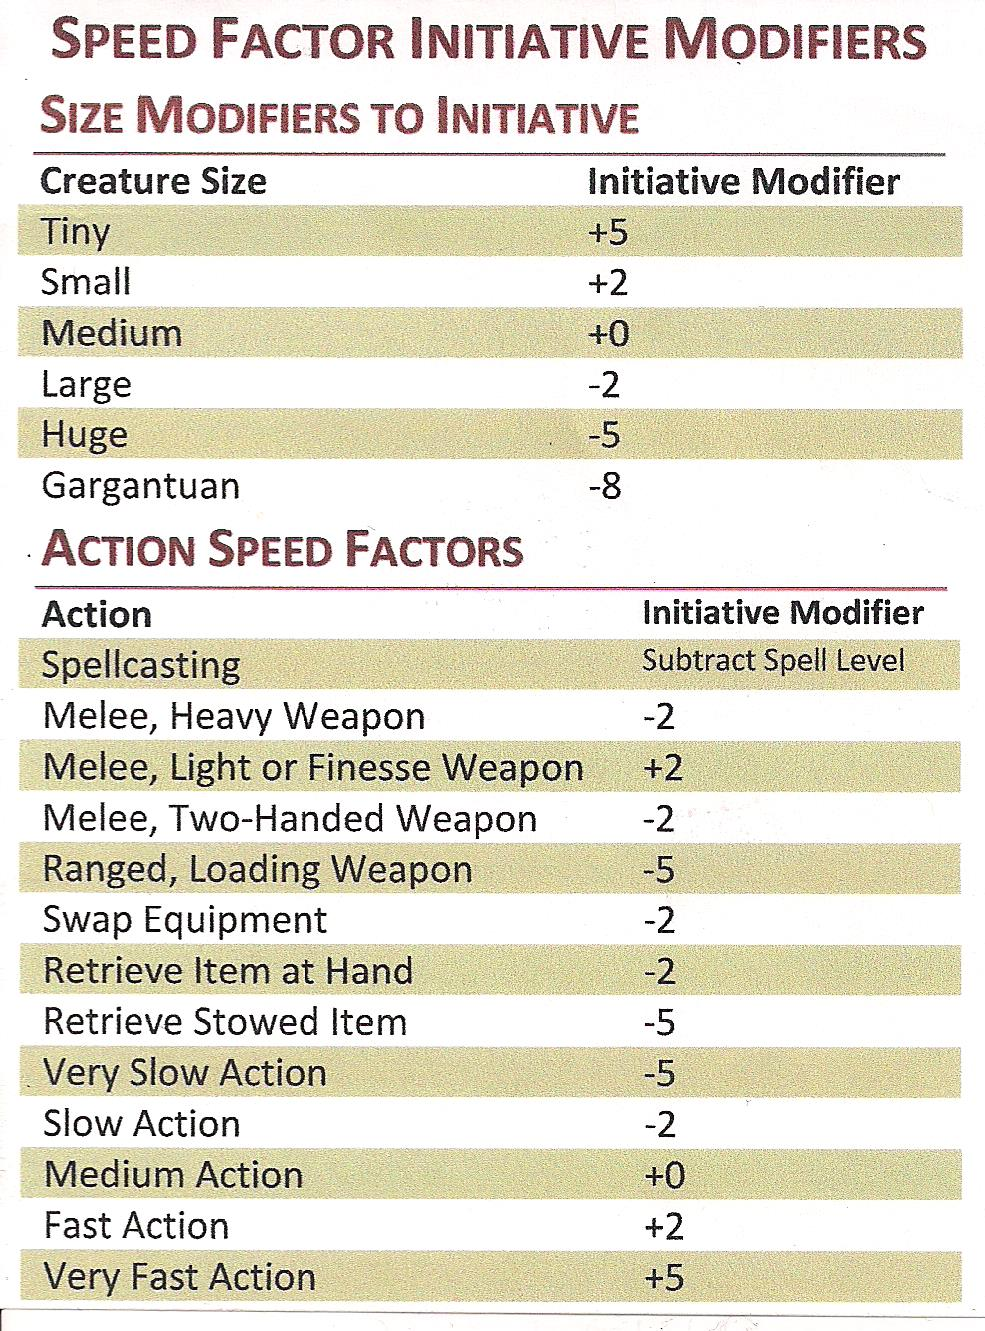
\includegraphics{img/speed-factor-initiative.jpeg}

\section{World map}
This is mostly as a note for me, but if it ever comes up on your next, a hex is 5 miles.
The PHB mentions that you can cover 18 / 24 / 30 miles a day at a slow / normal / fast pace,
  or 2 / 3 / 4 miles per hour.


\includegraphics[width=\linewidth,keepaspectratio=true]{img/maps/world-maps/Talaj.png}

\includegraphics[width=\linewidth,keepaspectratio=true]{img/maps/world-maps/Talaj2.png}


  \chapter{Plot}\label{ch:plot}

\chapter{Plot}\label{ch:plot}

\chapter{Plot}\label{ch:plot}

\input{story/00-preface/main}
\input{story/01-the-defense-of-celadirs-bastion/main}

The Stone of Shomah

The Celadonian has heard of a powerful artifact called the Stone of Shomah located in a ruin
  not far into the Tribal Wastes.
He doesn't know what power it holds, but knows that the Yuan-ti fear it above all things.


\chapter{Plot}\label{ch:plot}

\input{story/00-preface/main}
\input{story/01-the-defense-of-celadirs-bastion/main}

The Stone of Shomah

The Celadonian has heard of a powerful artifact called the Stone of Shomah located in a ruin
  not far into the Tribal Wastes.
He doesn't know what power it holds, but knows that the Yuan-ti fear it above all things.



The Stone of Shomah

The Celadonian has heard of a powerful artifact called the Stone of Shomah located in a ruin
  not far into the Tribal Wastes.
He doesn't know what power it holds, but knows that the Yuan-ti fear it above all things.


\chapter{Plot}\label{ch:plot}

\chapter{Plot}\label{ch:plot}

\input{story/00-preface/main}
\input{story/01-the-defense-of-celadirs-bastion/main}

The Stone of Shomah

The Celadonian has heard of a powerful artifact called the Stone of Shomah located in a ruin
  not far into the Tribal Wastes.
He doesn't know what power it holds, but knows that the Yuan-ti fear it above all things.


\chapter{Plot}\label{ch:plot}

\input{story/00-preface/main}
\input{story/01-the-defense-of-celadirs-bastion/main}

The Stone of Shomah

The Celadonian has heard of a powerful artifact called the Stone of Shomah located in a ruin
  not far into the Tribal Wastes.
He doesn't know what power it holds, but knows that the Yuan-ti fear it above all things.



The Stone of Shomah

The Celadonian has heard of a powerful artifact called the Stone of Shomah located in a ruin
  not far into the Tribal Wastes.
He doesn't know what power it holds, but knows that the Yuan-ti fear it above all things.



The Stone of Shomah

The Celadonian has heard of a powerful artifact called the Stone of Shomah located in a ruin
  not far into the Tribal Wastes.
He doesn't know what power it holds, but knows that the Yuan-ti fear it above all things.


  \chapter{Plot}\label{ch:plot}

\chapter{Plot}\label{ch:plot}

\chapter{Plot}\label{ch:plot}

\input{story/00-preface/main}
\input{story/01-the-defense-of-celadirs-bastion/main}

The Stone of Shomah

The Celadonian has heard of a powerful artifact called the Stone of Shomah located in a ruin
  not far into the Tribal Wastes.
He doesn't know what power it holds, but knows that the Yuan-ti fear it above all things.


\chapter{Plot}\label{ch:plot}

\input{story/00-preface/main}
\input{story/01-the-defense-of-celadirs-bastion/main}

The Stone of Shomah

The Celadonian has heard of a powerful artifact called the Stone of Shomah located in a ruin
  not far into the Tribal Wastes.
He doesn't know what power it holds, but knows that the Yuan-ti fear it above all things.



The Stone of Shomah

The Celadonian has heard of a powerful artifact called the Stone of Shomah located in a ruin
  not far into the Tribal Wastes.
He doesn't know what power it holds, but knows that the Yuan-ti fear it above all things.


\chapter{Plot}\label{ch:plot}

\chapter{Plot}\label{ch:plot}

\input{story/00-preface/main}
\input{story/01-the-defense-of-celadirs-bastion/main}

The Stone of Shomah

The Celadonian has heard of a powerful artifact called the Stone of Shomah located in a ruin
  not far into the Tribal Wastes.
He doesn't know what power it holds, but knows that the Yuan-ti fear it above all things.


\chapter{Plot}\label{ch:plot}

\input{story/00-preface/main}
\input{story/01-the-defense-of-celadirs-bastion/main}

The Stone of Shomah

The Celadonian has heard of a powerful artifact called the Stone of Shomah located in a ruin
  not far into the Tribal Wastes.
He doesn't know what power it holds, but knows that the Yuan-ti fear it above all things.



The Stone of Shomah

The Celadonian has heard of a powerful artifact called the Stone of Shomah located in a ruin
  not far into the Tribal Wastes.
He doesn't know what power it holds, but knows that the Yuan-ti fear it above all things.



The Stone of Shomah

The Celadonian has heard of a powerful artifact called the Stone of Shomah located in a ruin
  not far into the Tribal Wastes.
He doesn't know what power it holds, but knows that the Yuan-ti fear it above all things.


  \chapter{Plot}\label{ch:plot}

\chapter{Plot}\label{ch:plot}

\chapter{Plot}\label{ch:plot}

\input{story/00-preface/main}
\input{story/01-the-defense-of-celadirs-bastion/main}

The Stone of Shomah

The Celadonian has heard of a powerful artifact called the Stone of Shomah located in a ruin
  not far into the Tribal Wastes.
He doesn't know what power it holds, but knows that the Yuan-ti fear it above all things.


\chapter{Plot}\label{ch:plot}

\input{story/00-preface/main}
\input{story/01-the-defense-of-celadirs-bastion/main}

The Stone of Shomah

The Celadonian has heard of a powerful artifact called the Stone of Shomah located in a ruin
  not far into the Tribal Wastes.
He doesn't know what power it holds, but knows that the Yuan-ti fear it above all things.



The Stone of Shomah

The Celadonian has heard of a powerful artifact called the Stone of Shomah located in a ruin
  not far into the Tribal Wastes.
He doesn't know what power it holds, but knows that the Yuan-ti fear it above all things.


\chapter{Plot}\label{ch:plot}

\chapter{Plot}\label{ch:plot}

\input{story/00-preface/main}
\input{story/01-the-defense-of-celadirs-bastion/main}

The Stone of Shomah

The Celadonian has heard of a powerful artifact called the Stone of Shomah located in a ruin
  not far into the Tribal Wastes.
He doesn't know what power it holds, but knows that the Yuan-ti fear it above all things.


\chapter{Plot}\label{ch:plot}

\input{story/00-preface/main}
\input{story/01-the-defense-of-celadirs-bastion/main}

The Stone of Shomah

The Celadonian has heard of a powerful artifact called the Stone of Shomah located in a ruin
  not far into the Tribal Wastes.
He doesn't know what power it holds, but knows that the Yuan-ti fear it above all things.



The Stone of Shomah

The Celadonian has heard of a powerful artifact called the Stone of Shomah located in a ruin
  not far into the Tribal Wastes.
He doesn't know what power it holds, but knows that the Yuan-ti fear it above all things.



The Stone of Shomah

The Celadonian has heard of a powerful artifact called the Stone of Shomah located in a ruin
  not far into the Tribal Wastes.
He doesn't know what power it holds, but knows that the Yuan-ti fear it above all things.


  \chapter{Plot}\label{ch:plot}

\chapter{Plot}\label{ch:plot}

\chapter{Plot}\label{ch:plot}

\input{story/00-preface/main}
\input{story/01-the-defense-of-celadirs-bastion/main}

The Stone of Shomah

The Celadonian has heard of a powerful artifact called the Stone of Shomah located in a ruin
  not far into the Tribal Wastes.
He doesn't know what power it holds, but knows that the Yuan-ti fear it above all things.


\chapter{Plot}\label{ch:plot}

\input{story/00-preface/main}
\input{story/01-the-defense-of-celadirs-bastion/main}

The Stone of Shomah

The Celadonian has heard of a powerful artifact called the Stone of Shomah located in a ruin
  not far into the Tribal Wastes.
He doesn't know what power it holds, but knows that the Yuan-ti fear it above all things.



The Stone of Shomah

The Celadonian has heard of a powerful artifact called the Stone of Shomah located in a ruin
  not far into the Tribal Wastes.
He doesn't know what power it holds, but knows that the Yuan-ti fear it above all things.


\chapter{Plot}\label{ch:plot}

\chapter{Plot}\label{ch:plot}

\input{story/00-preface/main}
\input{story/01-the-defense-of-celadirs-bastion/main}

The Stone of Shomah

The Celadonian has heard of a powerful artifact called the Stone of Shomah located in a ruin
  not far into the Tribal Wastes.
He doesn't know what power it holds, but knows that the Yuan-ti fear it above all things.


\chapter{Plot}\label{ch:plot}

\input{story/00-preface/main}
\input{story/01-the-defense-of-celadirs-bastion/main}

The Stone of Shomah

The Celadonian has heard of a powerful artifact called the Stone of Shomah located in a ruin
  not far into the Tribal Wastes.
He doesn't know what power it holds, but knows that the Yuan-ti fear it above all things.



The Stone of Shomah

The Celadonian has heard of a powerful artifact called the Stone of Shomah located in a ruin
  not far into the Tribal Wastes.
He doesn't know what power it holds, but knows that the Yuan-ti fear it above all things.



The Stone of Shomah

The Celadonian has heard of a powerful artifact called the Stone of Shomah located in a ruin
  not far into the Tribal Wastes.
He doesn't know what power it holds, but knows that the Yuan-ti fear it above all things.



\chapter{Important Things}
\section{Magic Items}
\subsection{The Bottom Dollar}
Magic coin of an arbitrary denomination.
When in a container with other coins, it will always be the last coin withdrawn.
A creature that remembers any identifying characteristic of the coin
  (that would distinguish it from another in the container) can withdraw the coin without emptying
  the container on a successful Intelligence saving throw (DC 15).

This coin is a favorite among diviners who would like to keep track of a particular person.
By paying for a good with a Bottom Dollar, or `tipping' them for some small service, the diviner
  can track the coin to track their mark by proxy.

\end{document}
